% !TEX encoding = UTF-8 Unicode
\documentclass{beamer}
\usetheme{boxes}
%\usetheme[nototalframenumber,foot,logo]{uibk}
\usepackage{booktabs}
\usepackage{tikz}

\usepackage[czech]{babel}
\uselanguage{Czech}

\tikzstyle{block} = [
	rectangle, draw, fill=white,
	text width=4em,
	text centered,
	%rounded corners,
	minimum height=3.5ex,
	inner sep=0pt
]
\usetikzlibrary{arrows.meta,arrows}
\usetikzlibrary{patterns.meta}

% ------------------------------------------------------------------------
\title{Workshop: Neviditelný digitální inkoust}
%\titlegraphic{../../classes/Vertiefungsseminar/fig/VSSEC_title}
\subtitle{Úvodní prezentace}
\author{Martin Bene{\v s}}

% ------------------------------------------------------------------------
\begin{document}

\begin{frame}[plain]
\maketitle
\begin{tikzpicture}[overlay,remember picture]
\draw (current page.south west) node [above right, inner sep=.5cm] (uncover) {\includegraphics[height=1.2cm]{../img/uncover.png}};
\draw (current page.south east) node [above left, inner sep=.5cm] (uncover) {\includegraphics[height=1.2cm]{../img/uibk.png}};
\end{tikzpicture}
\end{frame}

% ------------------------------------------------------------------------
\begin{frame}<1>[label=agenda]
\frametitle{Agenda}
\begin{enumerate}
\item {\only<2>{\bfseries}O mně}
\item {\only<3>{\bfseries}Co je to steganografie?}
\item {\only<4>{\bfseries}Co je to steganalýza?}
\item {\only<5>{\bfseries}Struktura workshopu}
\item {\only<6>{\bfseries}Projekt Uncover}
\end{enumerate}
\end{frame}

%%%%%%%%%%%%%%%%%%%%%%%%%%%%%%%%%%%%%%%
\againframe<2>{agenda}

\begin{frame}
\frametitle{O mně}
\centering

\only<1>{
\includegraphics[height=25ex]{../img/gyrec_computers.jpg}%
\includegraphics[height=25ex]{../img/gyrec_garden.jpg}
\bigskip

Absolvent Gyrecu 2016
}

\only<2>{
%\includegraphics[height=20ex]{../img/vut_kunovsky.jpg}%
\includegraphics[height=30ex]{../img/vut_lamp.jpg}
\bigskip

Bc. z informatiky, FIT VUT, 2019
}


\only<3>{
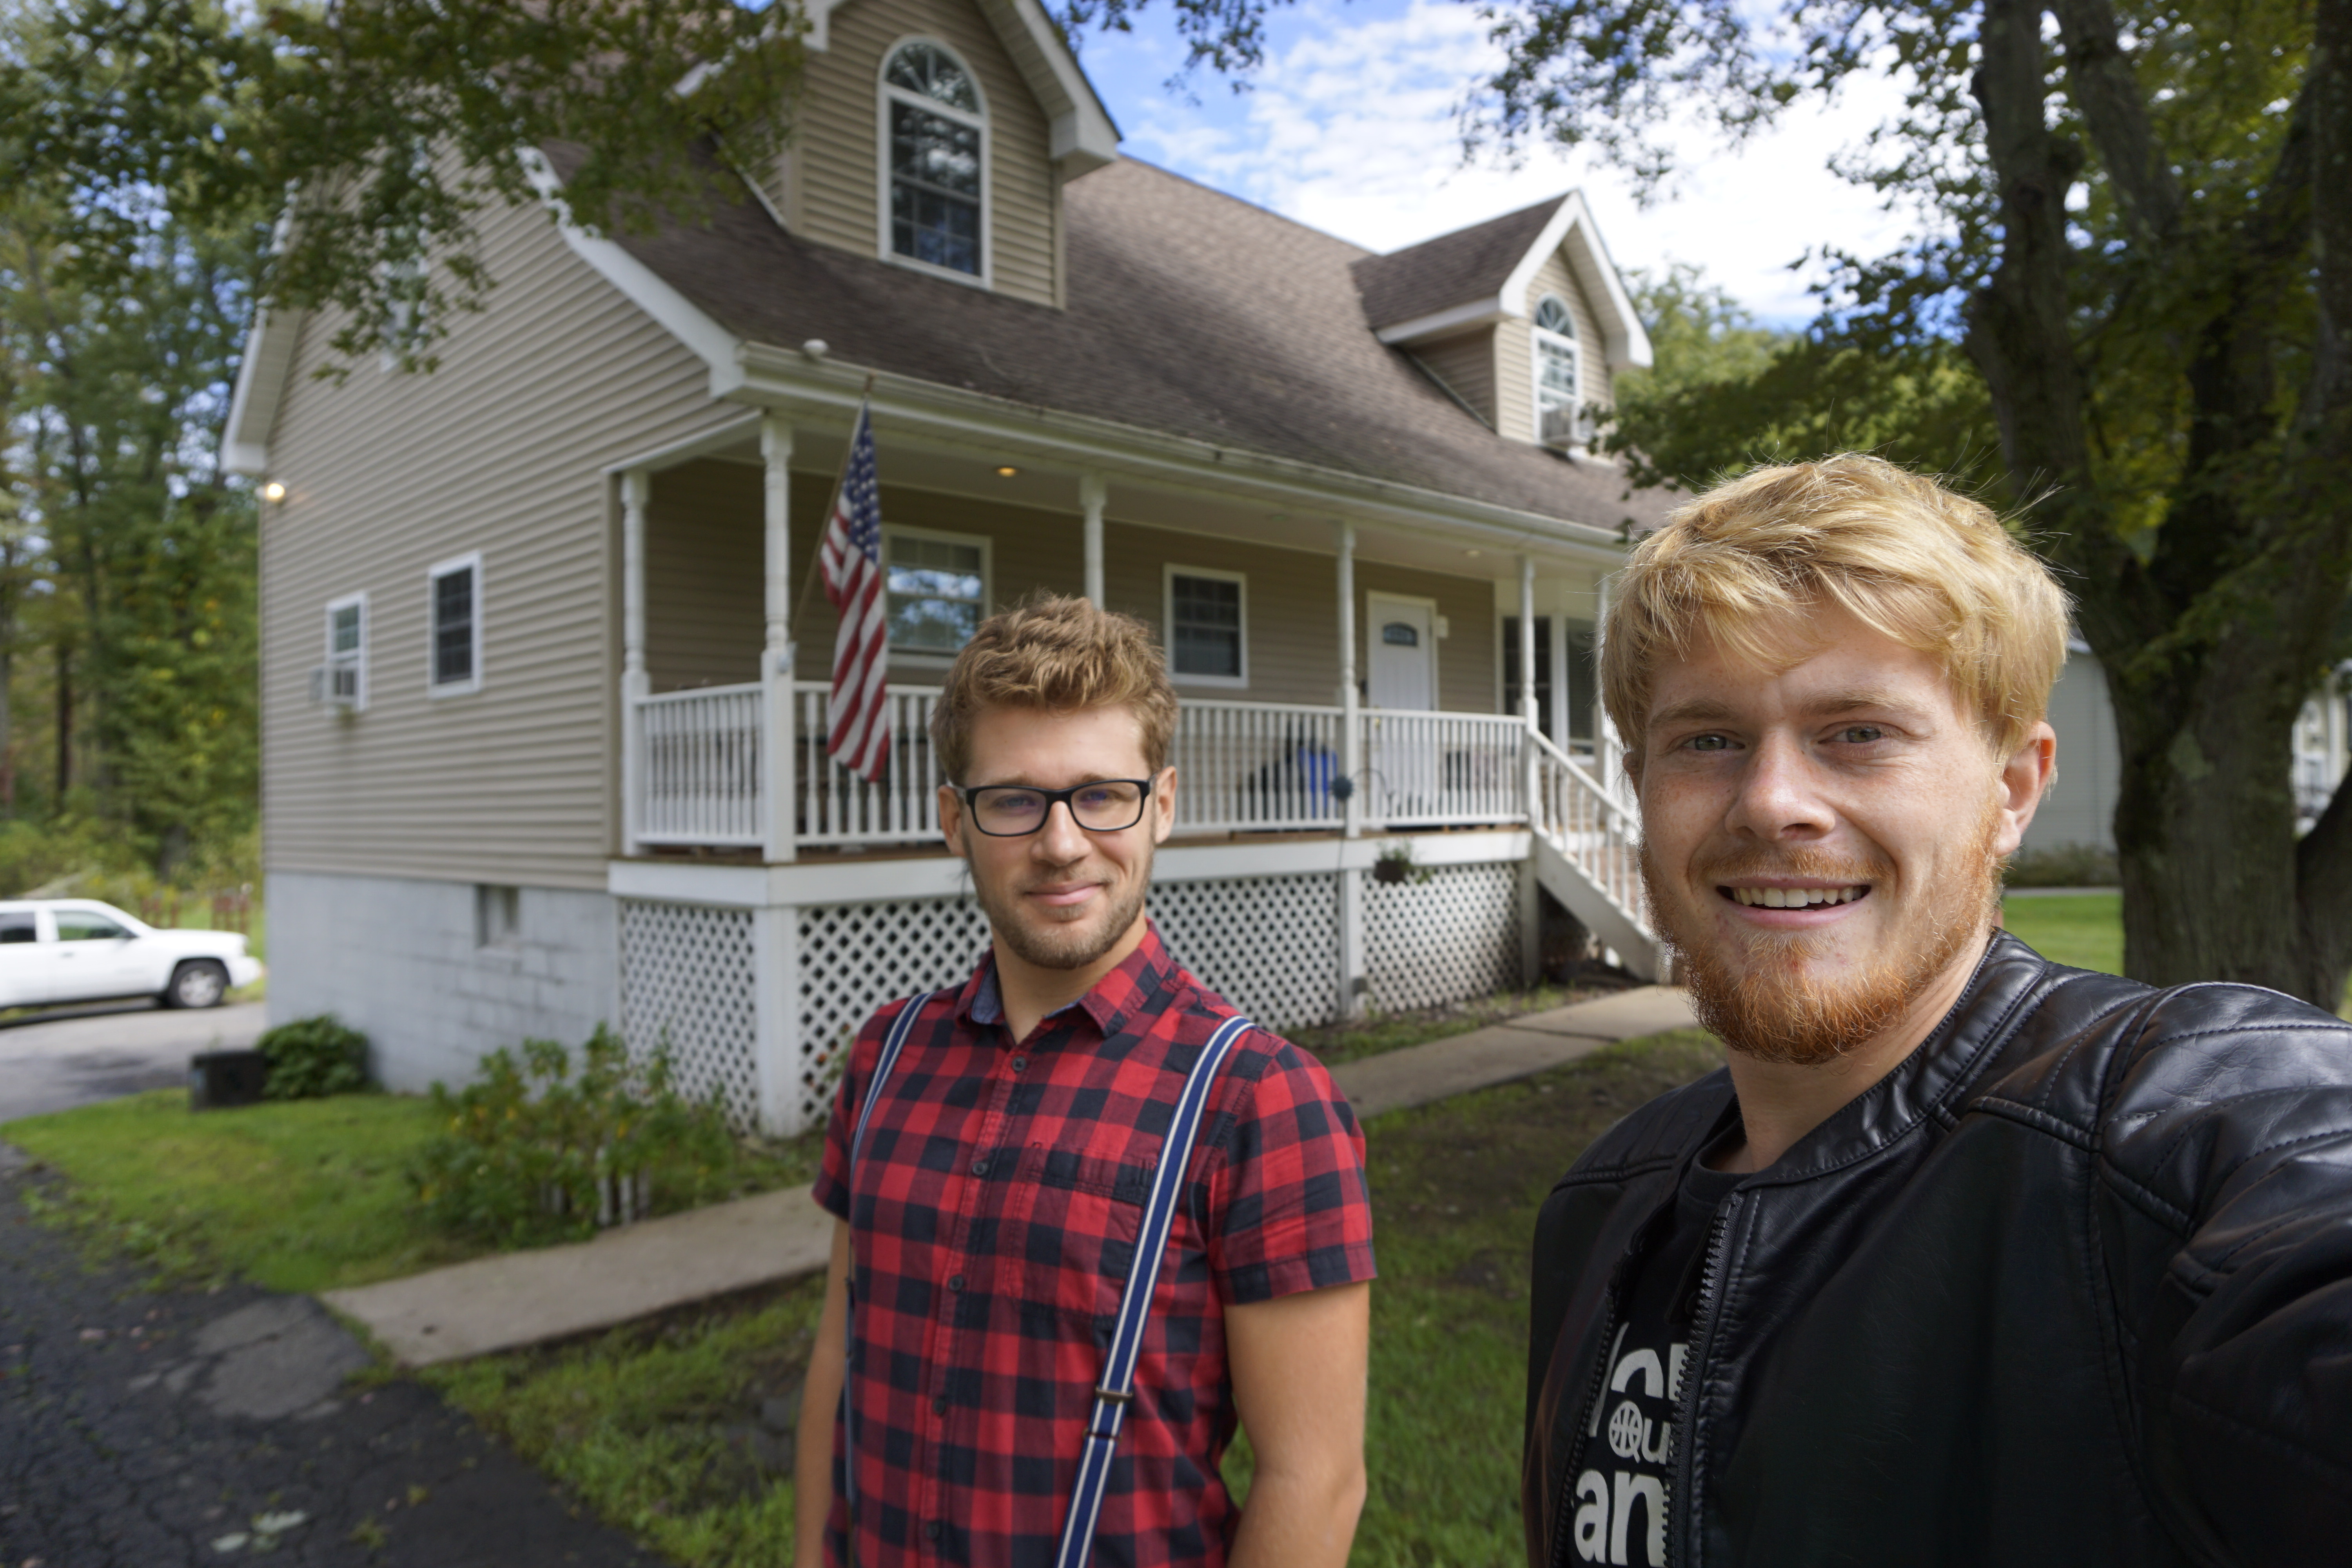
\includegraphics[height=20ex]{../img/usa_house.JPG}%
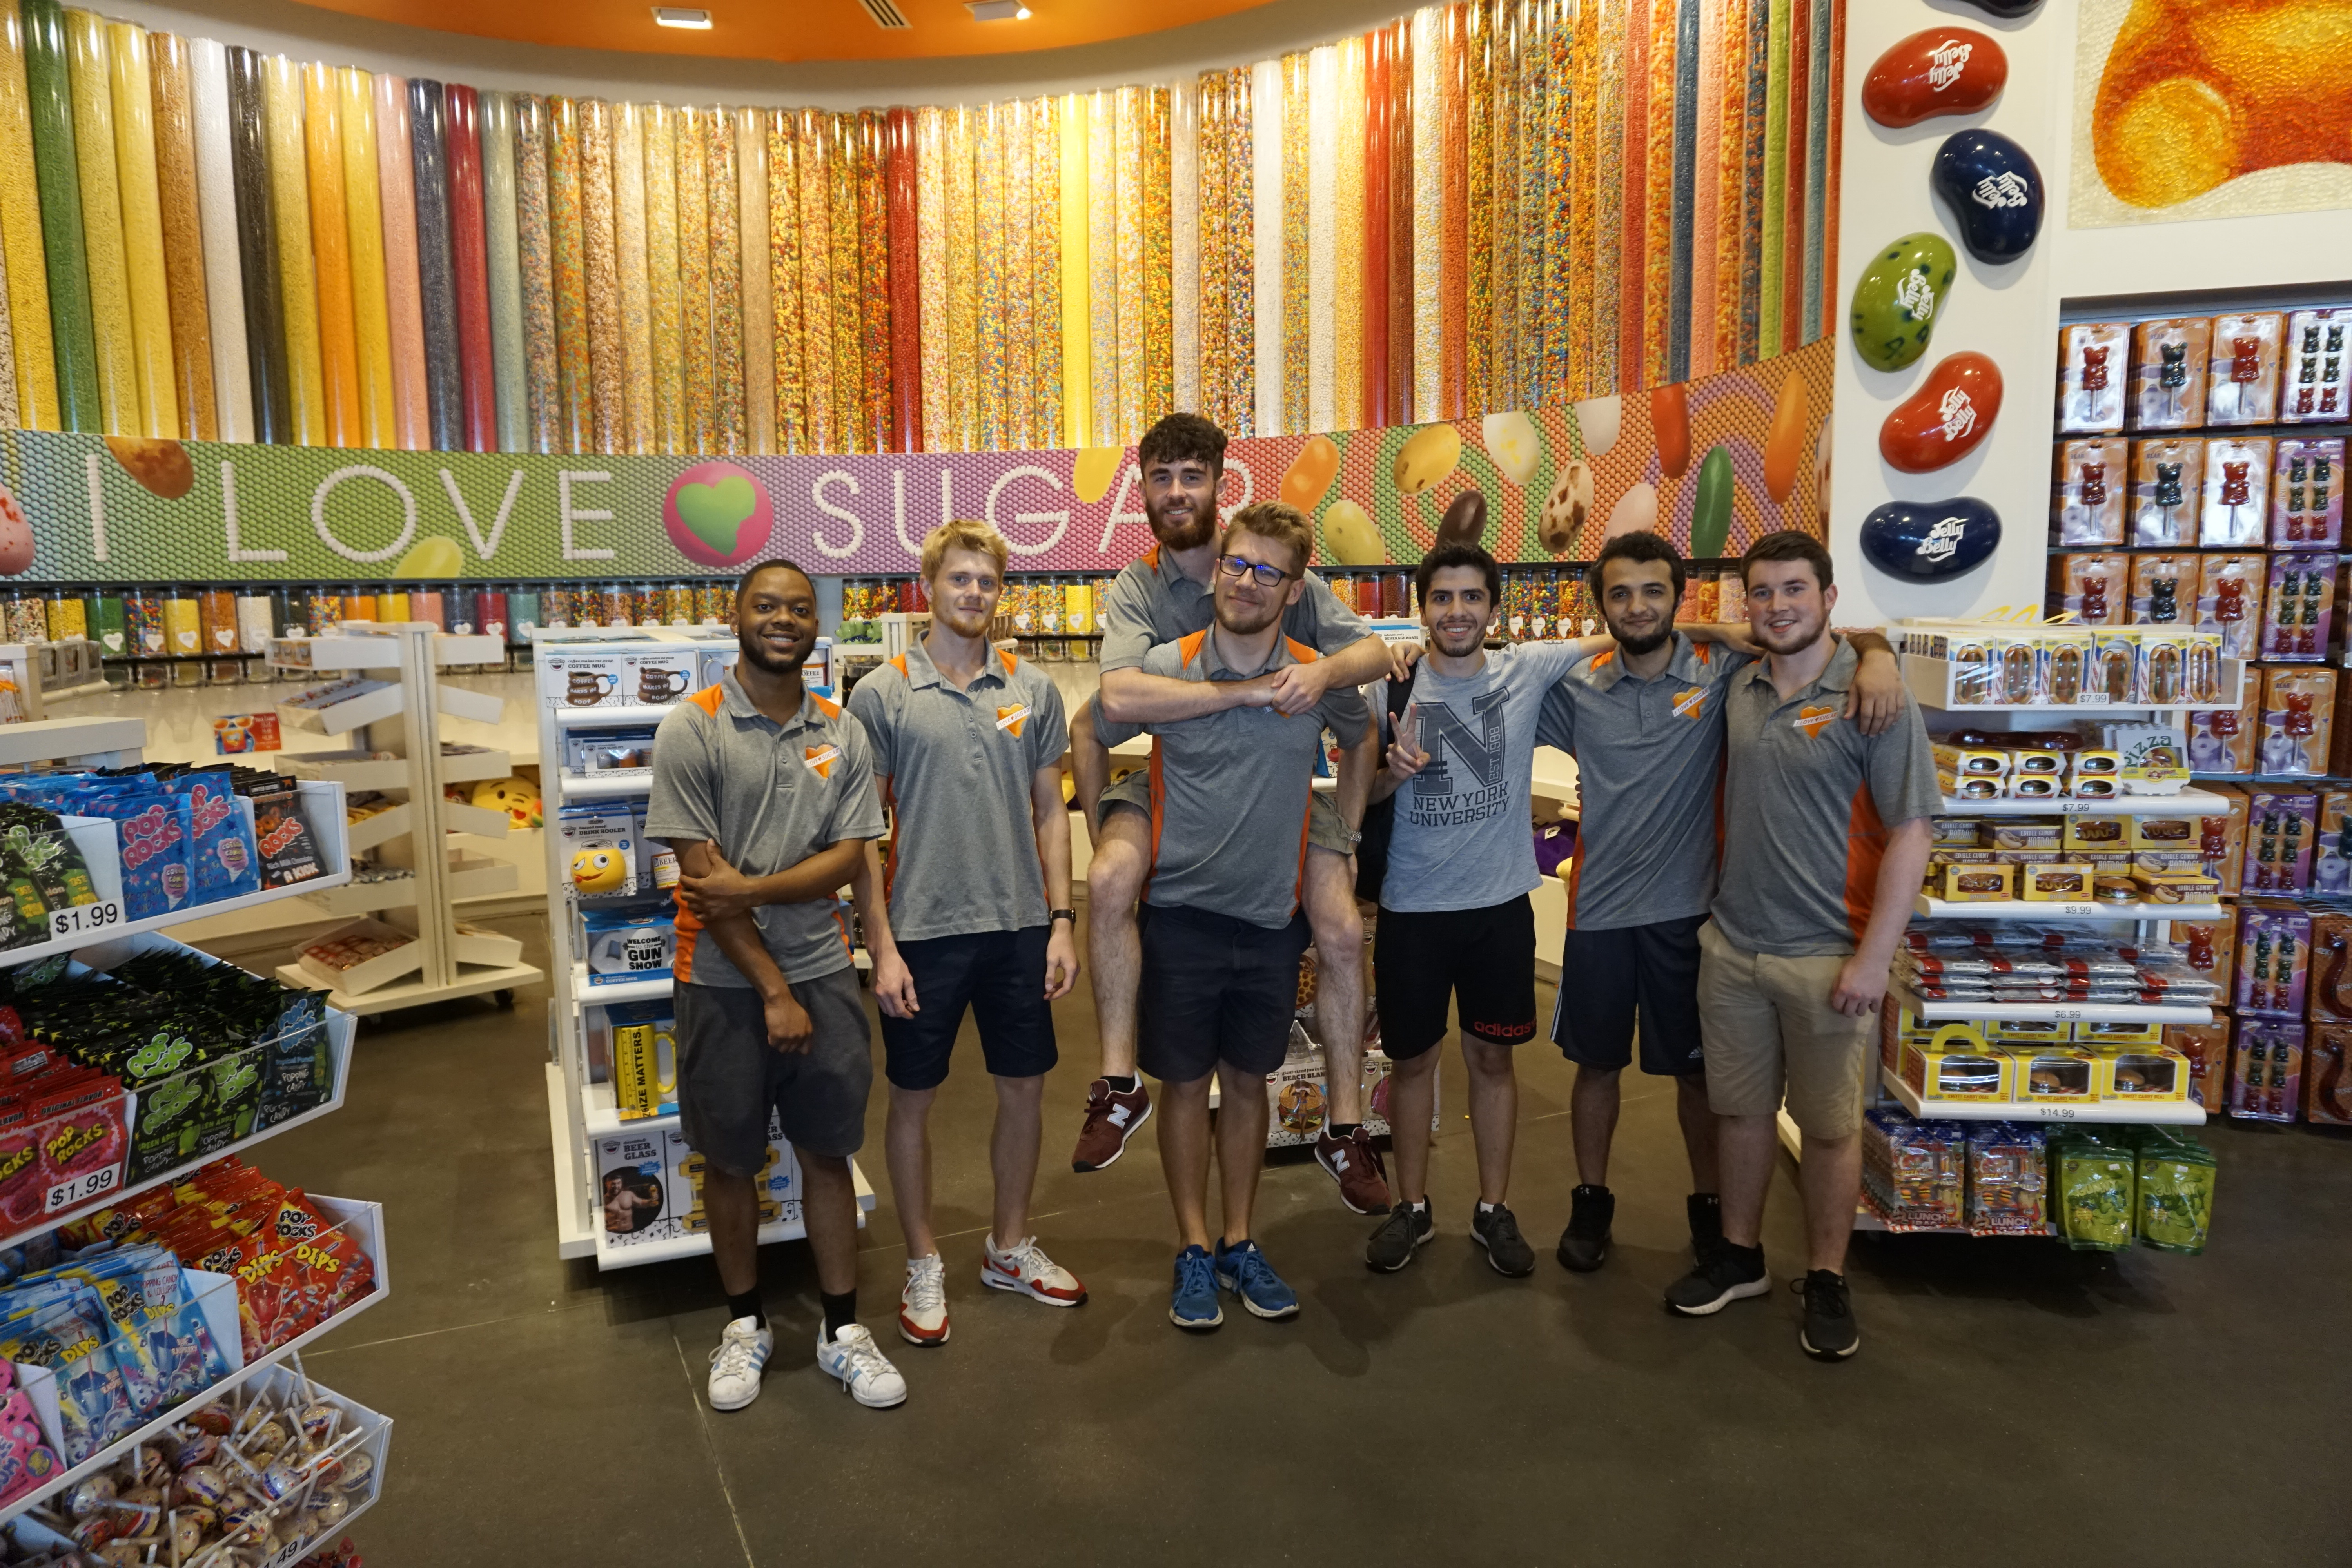
\includegraphics[height=20ex]{../img/usa_ilovesugar.JPG}
\bigskip

Work\&Travel v Myrtle Beach (USA), 2018
}

\only<4>{
\includegraphics[height=30ex]{../img/vorarlberg_karren.jpg}%
%\includegraphics[height=25ex]{../img/vorarlberg_fasching.jpg}
\bigskip

Erasmus+ na FH Vorarlberg (Rakousko), 2019
}

\only<5>{
\includegraphics[height=20ex]{../img/sweden_diploma.png}%
\includegraphics[height=20ex]{../img/sweden_work.jpg}
\bigskip

MSc. ze statistiky, Linköping Universitet (Švédsko), 2021
}

\only<6-7>{
%\begin{minipage}{.5\textwidth}
\centering
\includegraphics[height=20ex]{../img/innsbruck_ski.jpg}%
\includegraphics[height=20ex]{../img/innsbruck_wifs.jpeg}
%\end{minipage}%
%\begin{minipage}{.5\textwidth}
%\end{minipage}

\bigskip

[WIP] PhD. z informatiky, Innsbruck Universität (Rakousko), 2025
\bigskip

\onslide<7>{
\begin{center}
\textit{Steganografie $\cdot$ Steganalýza $\cdot$ Strojové učení}
\end{center}
}

}

\end{frame}


%%%%%%%%%%%%%%%%%%%%%%%%%%%%%%%%%%%%%%%
\againframe<3>{agenda}

\begin{frame}
\frametitle{Co je to steganografie?}

= ukrývání tajných zpráv do nenápadných, všedních objektů

\begin{itemize}
\item Kryptografie ukrývá smysl zprávy.
\item Steganografie ukrývá existenci zprávy.
\end{itemize}
\end{frame}

\providecommand{\iconKEY}[1]{\tikz[line width=1.2pt]{%
	\draw [yellow!90!black, -] (0,0) circle (.1);
	\draw [yellow!90!black, -] (-.1,0) -| (-.4,-.1);
	\draw [yellow!90!black, -] (-.1,0) -| (-.5,-.075);
	\draw [yellow!90!black, -] (-.1,0) -| (-.6,-.1);
	\draw (-.35,-.05) node [above, inner sep=2.5pt] {\scriptsize #1};
}}

\begin{frame}<1-8>[label=prisoner]
\frametitle{Problém vězně}
\centering

\begin{tikzpicture}
% steganographer
\path [fill=green!20!white] (-2, -1) rectangle ++(4, 3);
\path [fill=green!20!white] (4, -1) rectangle ++(4, 3);
\path (0, 1.5) node {\bf Alice\strut};
\path (0, 1) node (message1) {\scriptsize\texttt{Utečeme o půlnoci.}\strut};
% cover
\onslide<2->{
\path (-1.5, 0) node [inner sep=0pt, fill=black] (cover) {\includegraphics[height=3ex]{../img/monalisa.jpeg}}
	node [below=1.25ex] {\scriptsize Obálka\strut};
}
% embed
\onslide<3->{
\path (0, 0) node [block] (embed) {ukryj\strut};
\path [draw, -stealth] (message1.south) -- (embed.north);
\path [draw, -stealth] (cover.east) -- (embed.west)
	node [midway] (cover_center) {};
}

% steganalyst
\path (6, 1.5) node {\bf Bob\strut};
\onslide<6->{
\path (6, 0) node [block] (extract) {extrahuj\strut};
\path (6, 1) node (message2) {\scriptsize\texttt{Utečeme o půlnoci.}\strut};
\path [draw, -stealth] (extract.north) -- (message2.south);
}
\onslide<7>{
\path [draw, stealth-stealth, gray!70!white] (message1) to[out=20,in=160] [midway, above] node {\footnotesize stejná zpráva\strut} (message2);
}
% send connection
\onslide<4->{
\path [draw, -stealth] (embed.east) -- (extract.west)
	node [midway, above=2ex, inner sep=0pt] {\includegraphics[height=3ex]{../img/monalisa.jpeg}\strut}
	node [midway, above=0ex] {\scriptsize Stego\strut}
	node [midway] (stego) {};
}
\onslide<5>{
\path [draw, stealth-stealth, gray!70!white] (cover) to[out=-40,in=-140] [midway, below] node {\footnotesize nerozpoznatelné\strut} (stego);
}

% key
\onslide<8->{
\path (embed.south east) node [yellow!90!black] (embed_key){\iconKEY{}};
\path (extract.south west) node [yellow!90!black] (extract_key) {\iconKEY{}};
}
\onslide<8>{
\path [draw, stealth-stealth, gray!70!white] (embed_key) to[out=-20,in=-160] [midway, below] node {\footnotesize sdílený klíč\strut} (extract_key);
}

% steganalyst
\onslide<9->{
\path [fill=orange!20!white] (.5, -3.5) rectangle ++(5, 2);
\path (1.25, -2) node {\bf Eva\strut};
}
\onslide<10->{
\path (3, -2.5) node [block] (detect) {detekuj\strut};
\path [draw, -stealth] (detect.east) -- ++(.5, .5)
	node [pos=1, right] {\footnotesize\it obálka\strut};
\path [draw, -stealth] (detect.east) -- ++(.5, -.5)
	node [pos=1, right] {\footnotesize\it stego\strut};
}
\onslide<9->{
\path [draw, -stealth] (stego.center) -- (detect.north)
	node [pos=.65] (detect_center) {};
}
%
\end{tikzpicture}
\end{frame}


%%%%%%%%%%%%%%%%%%%%%%%%%%%%%%%%%%%%%%%
\againframe<4>{agenda}

\begin{frame}
\frametitle{Co je to steganalýza?}
= detekce steganografie, a to pomocí

\begin{itemize}
\item statistiky
\item strojového učení / umělé inteligence
\item digitální forenzní analýzy
\end{itemize}
\end{frame}

\againframe<9-10>{prisoner}

\begin{frame}
\frametitle{Účel steganalýzy}

\begin{itemize}
\item zjistit \underline{přítomnost} steganografie
\end{itemize}
\onslide<2>{
\begin{itemize}
\item poté zjišťujeme další informace (\textit{forenzní steganalýza})
\begin{itemize}
\item délka zprávy
\item steganografická metoda / nástroj
\item steganografický klíč (extrakce zprávy)
\item kryptografický klíč (dešifrování zprávy)
\item obsah zprávy
\end{itemize}
\end{itemize}
}
\end{frame}

\begin{frame}
\frametitle{Využití steganografie a steganalýzy}

\begin{itemize}
\item organizovaný zločin vs. kriminalisté
\item<2-> zpravodajské služby
\item<3-> disidenti vs. totalitní režim
\item<4-> stego-malware vs. antivirové programy
\end{itemize}
\bigskip

\onslide<5>{
= komunikace v nepřátelsky naladěném prostředí
}
\end{frame}

%%%%%%%%%%%%%%%%%%%%%%%%%%%%%%%%%%%%%%%
\againframe<5>{agenda}

\begin{frame}
\frametitle{Struktura workshopu}

\begin{enumerate}
\item Digitální obrázky
\begin{itemize}
\item Reprezentace v počítači
\item Zpracování obrázků
\end{itemize}
\item LSBr steganografie
\begin{itemize}
\item Sekvenční průchod
\item Permutovaný průchod
\end{itemize}
\item Základní steganalýza
\begin{itemize}
\item Analýza histogramu
\item $\chi^2$-test
\end{itemize}
\end{enumerate}
\end{frame}

%%%%%%%%%%%%%%%%%%%%%%%%%%%%%%%%%%%%%%%
\againframe<6>{agenda}

\begin{frame}
\frametitle{Oznámení o financování}
\centering

\begin{minipage}[t]{.5\textwidth}
\centering
\includegraphics[width=.9\columnwidth]{../img/uncover.png}
%\smallskip

\end{minipage}%
\begin{minipage}[t]{.5\textwidth}
\centering
\includegraphics[width=.7\columnwidth]{../img/uibk.png}
\end{minipage}

\begin{tikzpicture}[overlay,remember picture]
\draw (current page.south west) node [above right, inner sep=3pt] (uncover) {\includegraphics[height=.6cm]{../img/logo_eu.png}};
\path (uncover.east) node [right, align=left, font=\tiny, color=gray] {
Financováno z výzkumného a inovačního programu \\
EU Horizon 2020 pod grantovou smlouvou č. 101021687.};
\end{tikzpicture}

\end{frame}

\begin{frame}
\frametitle{Projekt Uncover}
\centering

\only<1-2>{
\begin{itemize}
\item Vývoj technologií pro detekci ukrytých informací.
\item<2-> Konsorcium 22 partnerů: univerzity, firmy, policie.
%\item<3-> Spolupráce univerzit, byznysu a policie.
\end{itemize}
\bigskip

\onslide<2>{
\begin{minipage}{.15\textwidth}\includegraphics[width=\columnwidth]{../img/logo_rma.png}\end{minipage}%
\begin{minipage}{.15\textwidth}\includegraphics[width=\columnwidth]{../img/logo_cnrs.png}\end{minipage}%
\begin{minipage}{.15\textwidth}\includegraphics[width=\columnwidth]{../img/logo_utt.png}\end{minipage}%
\begin{minipage}{.15\textwidth}\includegraphics[width=\columnwidth]{../img/logo_uibk.png}\end{minipage}%
\begin{minipage}{.15\textwidth}\includegraphics[width=\columnwidth]{../img/logo_ctu.png}\end{minipage}%
\begin{minipage}{.15\textwidth}\includegraphics[width=\columnwidth]{../img/logo_uvigo.png}\end{minipage}%

\begin{minipage}{.15\textwidth}\includegraphics[width=\columnwidth]{../img/logo_ovgu.png}\end{minipage}%
\begin{minipage}{.15\textwidth}\includegraphics[width=\columnwidth]{../img/logo_avast.png}\end{minipage}%
\begin{minipage}{.15\textwidth}\includegraphics[width=\columnwidth]{../img/logo_gradiant.png}\end{minipage}%
\begin{minipage}{.15\textwidth}\includegraphics[width=\columnwidth]{../img/logo_bka.png}\end{minipage}%
\begin{minipage}{.15\textwidth}\includegraphics[width=\columnwidth]{../img/logo_ertzaintza.png}\end{minipage}%
\begin{minipage}{.15\textwidth}\includegraphics[width=\columnwidth]{../img/logo_nicc.png}\end{minipage}%

\begin{minipage}{.15\textwidth}\includegraphics[width=\columnwidth]{../img/logo_nfi.png}\end{minipage}%
\begin{minipage}{.15\textwidth}\includegraphics[width=\columnwidth]{../img/logo_pol.png}\end{minipage}%
\begin{minipage}{.15\textwidth}\includegraphics[width=\columnwidth]{../img/logo_plusethics.png}\end{minipage}%
\begin{minipage}{.15\textwidth}\includegraphics[width=\columnwidth]{../img/logo_thales.png}\end{minipage}%
\begin{minipage}{.15\textwidth}\includegraphics[width=\columnwidth]{../img/logo_zitis.png}\end{minipage}%
\begin{minipage}{.15\textwidth}\includegraphics[width=\columnwidth]{../img/logo_npn.png}\end{minipage}%

\begin{minipage}{.15\textwidth}\includegraphics[width=\columnwidth]{../img/logo_synyo.png}\end{minipage}%
\begin{minipage}{.15\textwidth}\includegraphics[width=\columnwidth]{../img/logo_cta.png}\end{minipage}%
\begin{minipage}{.15\textwidth}\includegraphics[width=\columnwidth]{../img/logo_suneris.png}\end{minipage}%
\begin{minipage}{.15\textwidth}\includegraphics[width=\columnwidth]{../img/logo_nbi.png}\end{minipage}%
\begin{minipage}{.15\textwidth}\includegraphics[width=\columnwidth]{../img/logo_lpr.png}\end{minipage}%
}
}

\only<3>{
\includegraphics[width=1.\columnwidth]{../img/uncover_meeting.jpeg}
}
\end{frame}


\end{document}
